\documentclass{article}

\usepackage[utf8]{inputenc}
\usepackage[brazil]{babel}
\usepackage[a4paper, left=3cm, right=2cm, top=3cm, bottom=2cm]{geometry}
\usepackage{indentfirst}
\usepackage[]{graphicx}
\usepackage{amsmath}
\usepackage{float}
\usepackage{lipsum}
\usepackage{xcolor}
\usepackage{fancyvrb}
\usepackage{verbatimbox}

\catcode`>=\active %
\catcode`<=\active %
\def\openesc{\color{red}}
\def\closeesc{\color{black}}
\def\vbdelim{\catcode`<=\active\catcode`>=\active%
\def<{\openesc}
\def>{\closeesc}}
\catcode`>=12 %
\catcode`<=12 %

\newcommand{\assignment}{Trabalho 1}
\newcommand{\duedate}{23 de Abril}

\title{
    Relatório do \assignment \\
    % Subtítulo
    Pipeline de Processamento de Dados - Simulação de Rodovias
}
\author{
    Breno Marques Azevedo \\
    Bruno Pereira Fornaro \\
    Luis Fernando Laguardia \\
    Vinicius Hedler \\
    Vanessa Wille 
}
\date{\today}

\begin{document}
    \noindent
    Fundação Getulio Vargas\hfill\\
    Computação Escalável\hfill\textbf{\assignment}\\
    Prof.\ Thiago Pinheiro de Araújo\hfill\textbf{Entrega:} \duedate\\
    \smallskip\hrule\bigskip

    {\let\newpage\relax\maketitle}
    \maketitle

    \section{Introdução}
    Neste trabalho iremos implementar um pipeline de processamento de dados
    para um sistema de monitoramento de rodovias, seguindo o modelo ETL 
    (Extract, Transform, Load) e utilizando os mecanismos apresentados
    em aula para executar de forma concorrente e paralela.

    \section{Modelagem}
    Segue abaixo a divisão do trabalho entre os membros do grupo:
    \begin{figure}[H]
        \centering
        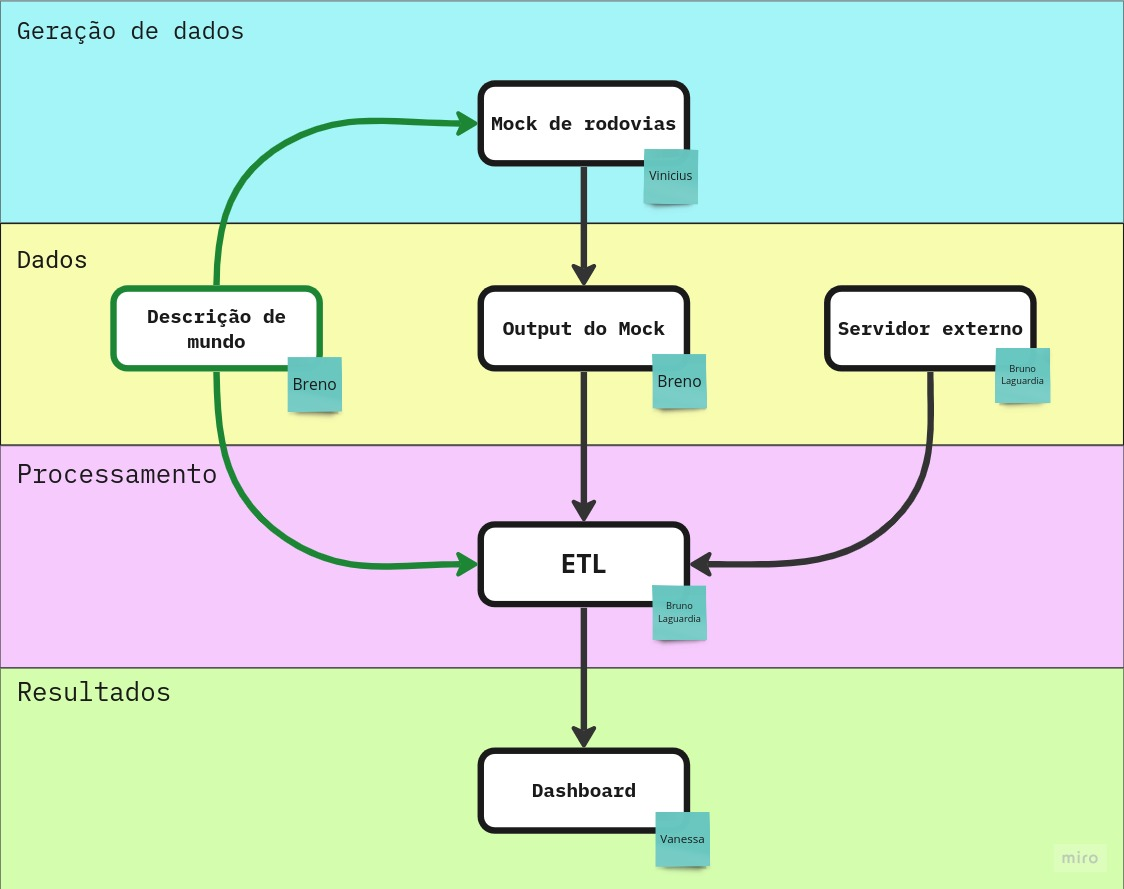
\includegraphics[width=13cm]{figs/modelagem.jpg}
        \caption{Modelagem do Trabalho}
        \label{fig:modelagem}
    \end{figure}

    Inicialmente, definimos bem como seria o funcionamento do Mock, a fim de projetar
    como o que esperar durante o processamento dos dados. Isso nos ajudou a 
    compartimentalizar o trabalho de forma relativamente independente. Contudo, ainda
    mantivemos uma comunicação constante entre os membros do grupo. Realizamos reuniões
    periódicas para discutir como implementar cada parte do trabalho, falar sobre o 
    andamento do projeto e debater problemas que surgiam durante o desenvolvimento.

    \subsection*{Mock}
    Primeiramente, uma vez que implementar um sistema de monitoramento de rodovias
    não é o objetivo do trabalho, criamos um Mock que imita o comportamento que um sistema desse tipo teria.
    O Mock simula uma rodovia e os carros que passam por ela, bem como as colisões que podem ocorrer.
    Por conta disso, decidimos que o Mock teria cada uma dessas três classes.
    
    Cada carro possui uma série de atributos, tais como placa, modelo, velocidades máxima e mínima, 
    acelerações máxima e mínima, uma probabilidade de colisões e uma probabilidade de trocar de faixa.
    Dessa forma, é possível que o carro siga em frente, troque de faixa ou cause algum tipo de colisão.

    Por sua vez, cada rodovia é composta por um comprimento, número de faixas em cada sentido,
    um limite de velocidade e uma lista que armazena uma lista de carros e outra lista de colisões.

    Por fim, as colisões são representadas por uma lista de carros que colidiram e as respectivas
    contagens desses carros que colidiram.

    \subsection*{Mock - Vinicius}
    O arquivo `mock.py' contém o mock, um simulador de rodovias. É ele que irá simular as rodovias,
    carros e suas colisões, para então gravar os dados das simulações de maneira que o ETL possa ser alimentado.
    Consiste de três arquivos: `world\_creator.py', `world.txt' e `mock.py', além do diretório `roads' onde é salvo
    o output da simulação. Em `mock.py' há quatro classes relevantes: `World', `Road', `Car' e `Collision'.

    \subsubsection*{world\_creator}
    Antes de poder executar `mock.py' é necessário\ executar `world\_creator.py'. Este script irá criar o arquivo
    `world.txt'. Em `world.txt', cada linha representa os dados de inicialização de uma rodovia distinta, e tais
    dados estão dispostos na seguinte ordem:

    * nome da rodovia
    * quantidade de vias no sentido principal
    * quantidade de vias no sentido oposto
    * comprimento da via
    * limite de velocidade da via
    * probabilidade de um novo carro entrar em alguma via a cada ciclo
    * probabilidade de um carro mudar de via arbitrariamente
    * probabilidade de um carro não tentar evitar uma colisão
    * velocidade mínima dos carros
    * velocidade máxima dos carros
    * aceleração mínima dos carros
    * aceleração máxima dos carros
    * quantidade de ciclos para uma colisão ser removida

    Os dados de `world.txt' são escolhidos aleatóriamente em `world\_creator.py', dentro de intervalos selecionados.

    \subsubsection{World}
    Assim que o arquivo `mock.py' é executado, é rodada a função `create\_world'. Esta função irá criar uma instância
    da classe `World' com rodovias contendo os dados em `world.txt'. Com as rodovias criadas, a instância de `World'
    entrará em loop.

    Em seu loop, `world' irá, para cada rodovia, executar um ciclo e então gravar seus dados em um novo arquivo no
    diretório `temp'. O nome do arquivo será o ciclo atual que esta sendo executado + `.txt'. Uma vez que o ciclo
    atual foi executado para todas as rodovias, o arquivo será transferido para o diretório `roads'.


    \subsubsection{Road}
    Quando for criada, uma rodovia recebe os parâmetros mencionados anteriormente e os salva. Além disto, cria
    uma lista 2D dentro de si contendo as vias. Ao ser inicializada, cada via será uma lista de None com comprimento
    igual ao comprimento da rodovia.

    O ciclo da rodovia começa por pedir para cada carro dentro de si decidir se irá acelerar e/ou mudar de pista.
    Isto é feito atravessando cada uma das células da rodovia, primeiro pela posição horizontal (pelo comprimento
    da rodovia), começando pelo final da rodovia, e depois pela posição vertical (pelas vias da rodovia). Isto é
    feito porque há casos em que se o carro mais a frente se mover primeiro, o carro mais atrás não irá colidir com
    ele.

    Quando um carro se move, há três possibilidades:
    - O carro se moveu sem problemas. Neste caso, apenas é criada referência ao objeto do carro na nova posição
    - O carro se move para uma posição além do fim da via. Neste caso nada acontece além do passo de remoção
    - O carro se move para uma posição onde já há um carro ou colisão. Neste caso é  criada uma nova colisão ou o
    carro é adicionado à colisão já existente no local.
    
    Independente do caso, o valor na posição antiga do carro é substituído por None.
    
    Há também o caso em que uma célula não contém um carro, mas sim uma colisão. Neste caso, o contador da colisão
    é reduzido em um e, se chegar a zero, a colisão é removida.
    Após os objetos em cada uma das células ter tido sua chance de agir, é decidido aleatoriamente para cada via se
    um carro irá aparecer nela. Ou seja, em cada rodovia é escolhido um valor entre 0 e 1. Se o valor for menor
    que o atributo `car\_spawn\_prob' (float entre 0 e 1), um novo carro é criado no começo de tal via.
    

    \subsubsection{World}

    \subsubsection{Road}
    Os objetos de carro são criados em algum objeto `Road'. Assim, recebem de `Road' os seguintes atributos:

    * via em que estão
    * velocidade mínima
    * velocidade máxima
    * aceleração mínima
    * aceleração máxima
    * chance de trocar de via arbitrariamente
    * chance de não evitar uma colisão

    Receber estes atributos diretamente da rodovia significa que eles são iguais para todos os carros (com
    exceção do atributo via). Note que os atributos de velocidade e aceleração são referentes à mecânica do
    carro, e o carro sempre irá respeitá-los, ao contrário do limite de velocidade da rodovia, que pode ser
    desrespeitado.

    A função principal de um carro e `decide\_movement'. Nesta função, um carro pede à rodovia para que verifique
    se o caminho está livre, começando em sua posição atual e terminando em sua posição atual mais sua velocidade.
    Se o caminho estiver livre, o carro o percorre. Há de se notar que o carro na verdade não se move sozinho, o que
    ele faz é mudar seus valores de posição e então pedir à rodovia que o mova dentro de seu objeto `road'.

    Caso o caminho não esteja livre, o carro tenta mudar de via. Para mudar de via ele escolhe aleatoriamente entre
    as vias da esquerda e da direita, considerando apenas as que estão livres. Caso o carro tenha conseguido mudar
    de via, ele verifica novamente se o caimnho à frente está livre. Agora, se o caminho ainda estiver bloqueado, o
    carro desacelera o máximo que conseguir. Sempre que as medidas para evitar uma colisão (mudar de via e desacelerar)
    são tomadas, é escolhido um float entre 0 e 1, e se este for menor que `risk', as medidas não são tomadas e o
    carro irá forçar uma colisão.

    Antes de um carro utilizar sua função `decide\_movement', ele acelera, adicionando um valor aleatório entre sua
    aceleração mínima e aceleração máxima. Caso sua nova velocidade esteja abaixo de sua velociade mínima, a velocidade
    do carro é atualizada para ser igual a sua mínima. O mesmo ocorre para sua velocidade máxima.
    
    \subsubsection*{Collision}
    Quando é criado, um objeto `Collision' recebe os dois carros envolvidos na colisão e o valor máximo do contador de
    remoção de colisão da rodovia em que ocorreu. A cada ciclo este contador decresce em um, e quando chegar a zero a
    colisão é removida da rodovia. Caso um carro colida em uma colisão já existente, o carro simplesmente é adicionado
    aos carros envolvidos na colisão e removido da rodovia.

    \subsection*{ETL}
    \lipsum[1]

    \subsection*{Dashboard}
    \lipsum[2]

    \section{Mock}
    Como mencionado acima, o Mock é uma simulação de um sistema de monitoramento de rodovias.
    Ele é composto pela rodovia, os carros e as colisões. É possível visualizar a simulação
    ocorrendo a cada ciclo. Além disso, ele gera como saída um arquivo com o nome da rodovia
    observada, os carros que passam por ela e suas respectivas posições - o número da via e 
    distância percorrida.
    
    Segue um exemplo de simulação do Mock:

    \begin{verbnobox}[\vbdelim]
2                                                     <9>                                                                                                           2                                                                                                                                        
 2                                                        <9>                 
                               2                                            
------------------------------------------------------------------------------------
                                                 -4                         
                                                 <8>                        -3         
             -2
    \end{verbnobox}
    
    Acima, temos uma simulação de uma rodovia com 3 faixas em cada sentido. Os números representam
    as acelerações. O sinal negativo representa que esses carros estão indo no sentido oposto ao
    da faixa de cima. Já os números em vermelho são as contagens regressivas das colisões, que são
    atualizadas a cada ciclo.

    Além disso, a simulação também gera um arquivo de output que contém o nome da rodovia observada,
    as placas dos carros que passam por ela e suas respectivas posições a cada ciclo. A posição do
    veículo é representada por um par ordenado com o número da via e a distância percorrida.
    Segue abaixo um exemplo de arquivo de output, referente à simuação acima:

    \begin{verbatim}
> BR-286
DQF9D30 000,000
TWB3V34 001,001
EOI9E67 002,010
DWQ5P39 003,017
JYX8N25 004,007
IFK9V68 005,034
    \end{verbatim}

    O output em questão será usado como entrada para o processo de ETL.

    \section{ETL}

    \section{Dashboard}

    \section{Problemas e Soluções}

    \section{Conclusão}

\end{document}
